\section{COMPUTAÇÃO EVOLUCIONÁRIA}
\label{sec:computacaoevolucionaria}

A \ac{CE} é um paradigma na área de Inteligência Artificial 
que tem como inspiração a teoria da evolução biológica de Charles Darwin. A teoria de Darwin afirma que a evolução 
dos seres vivos resulta dos processos de seleção, recombinação, reprodução e mutação onde a cada geração apenas sobrevivem os 
indivíduos mais “aptos” da população \citep{Darwin1859}. 

Tradicionalmente a \ac{CE} é composta pelas seguintes áreas ou \ac{AE}:
\begin{itemize}
  	\item {\ac{EE} \citep{Schw75}}
  	\item {\ac{PE} \citep{Fogel1962}} 
	\item {\ac{AG} \citep{Holland1975}}
	\item {\ac{PG} \citep{Koza1992}}
\end{itemize}

Todas estas técnicas partilham do comum objetivo de produzir sistemas automáticos para a resolução de problemas de otimização ou de pesquisa num 
espaço de soluções possíveis. A \tableref{Tabela111} mostra a analogia de alguns dos termos mais utilizados em \ac{CE}.

\begin{table}[H]
    \begin{tabular}{ll}%
    \toprule
    \textbf{Evolução darwiniana} & \textbf{\ac{CE}}\\ 
    \midrule
    Ambiente				& Problema\\ 
    Indivíduo				& Solução candidata\\ 
    Aptidão	(\emph{fitness})	& Qualidade da solução\\
    \bottomrule
    \end{tabular}
    \centering
    \caption{Analogia entre a evolução darwiniana e a \ac{CE}}
    \label{Tabela111}
\end{table}

Os \acp{AG} são o tipo de \ac{AE} mais antigo e mais estudado. Num \ac{AG}, um indivíduo 
é representado por uma cadeia fixa de caracteres. Cada indivíduo representa uma solução para o problema em questão e a sua 
capacidade de resolver tal problema é determinada por uma 
função de aptidão\footnote{Também chamada de função de \emph{fitness}, função-objetivo ou função de custo. Ao longo deste relatório 
será utilizado o termo: função de \emph{fitness}.}.
Ao longo das gerações (ou iterações) do algoritmo, uma nova população é criada contendo os melhores indivíduos da 
geração anterior e outros indivíduos que são produzidos por cruzamento e mutação \citep{mitchell1998introduction}. 
A \figref{Figura111} ilustra o esquema de funcionamento geral de um \ac{AG}.

\begin{figure}[H]
	\centering
	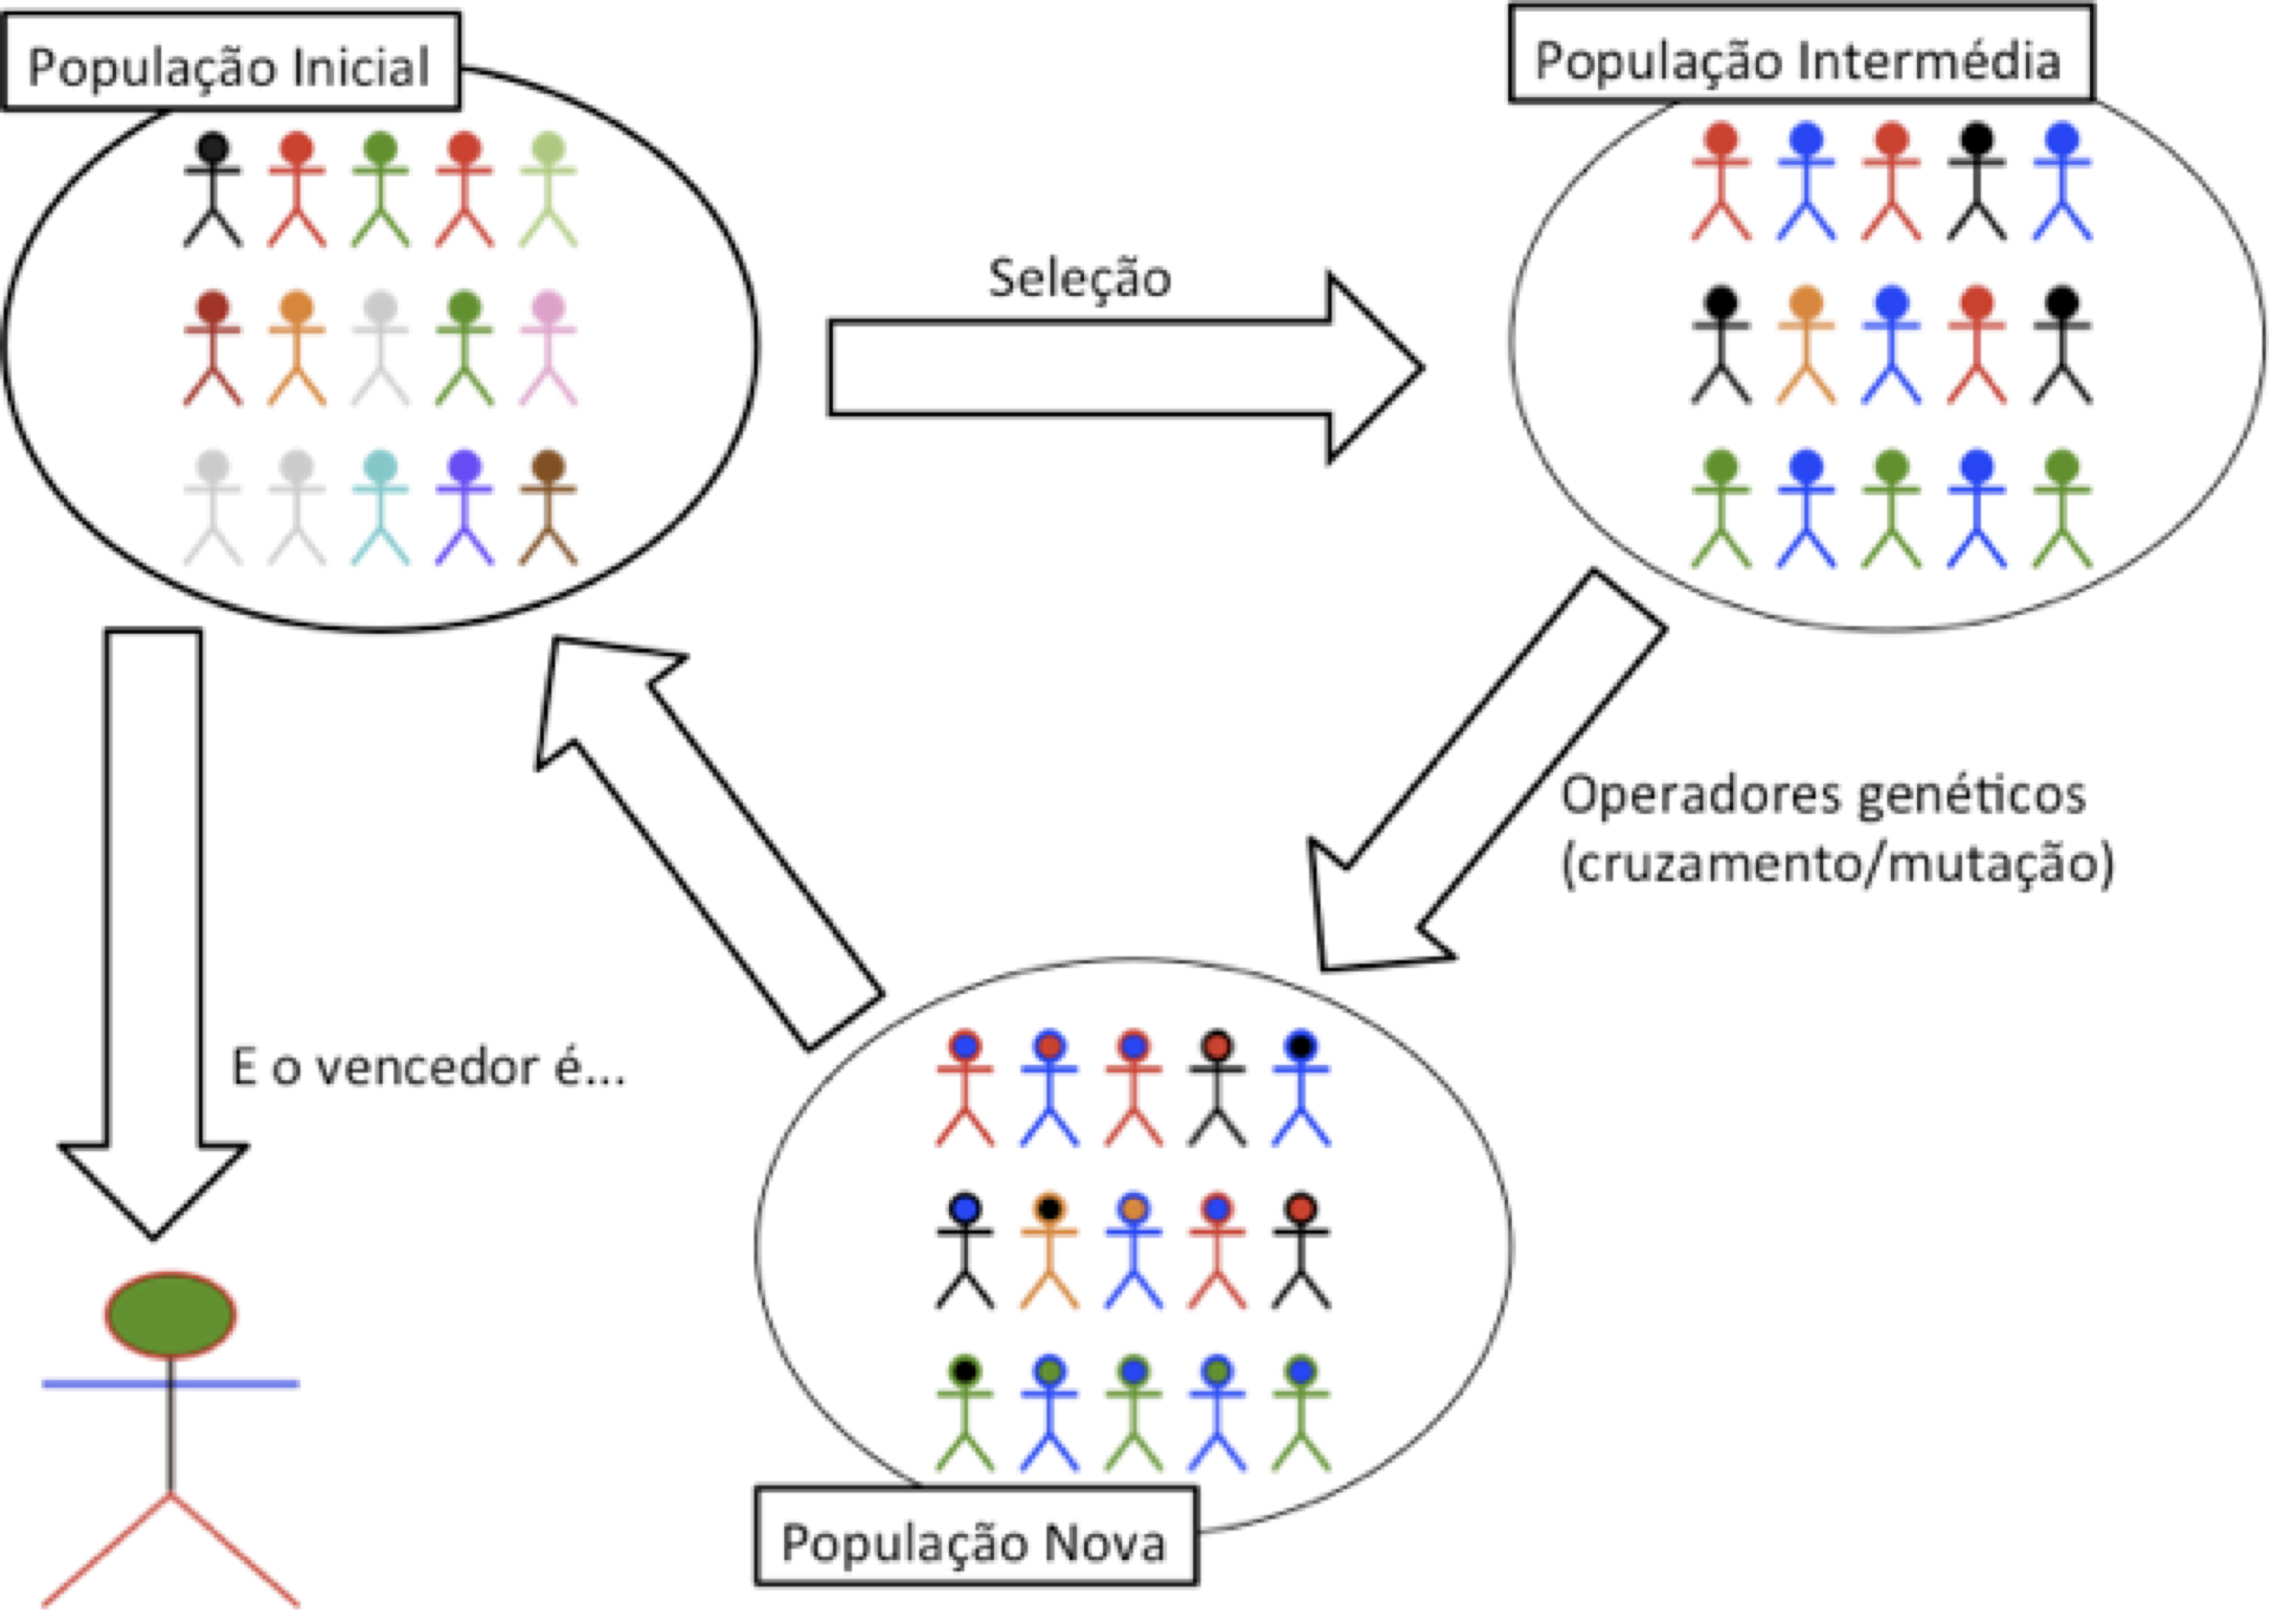
\includegraphics[width=0.75\textwidth]{figures/1}
	\caption{Funcionamento geral de um \ac{AG} padrão}
	\label{Figura111}
\end{figure}

Para a execução de um \ac{AG} deve ser definido à partida o conjunto de caracteres que representam os indivíduos. 
De seguida, é definido também o tamanho $L$ de cada indivíduo, a função de \emph{fitness} e outros parâmetros fundamentais
(e.g. quantidade de indivíduos na população, número máximo de gerações, etc.) \citep{Holland1975}. 
Ao representar os indivíduos com os caracteres binários $0$ e $1$, o tamanho do espaço de pesquisa (ou o conjunto de soluções
possíveis) será $2^L$ ou seja, existirão $2^L$ 
indivíduos diferentes.

O processo, tal como ilustrado na \figref{Figura111}, começa com a criação aleatória de uma população de tamanho $p$. 
Posteriormente o algoritmo entra num ciclo (geração) onde a cada iteração todos os indivíduos são avaliados e recebem um valor de \emph{fitness}. 
Alguns indivíduos são selecionados e copiados para a geração intermédia. Este processo é repetido $p$ vezes para que no final a 
população intermédia tenha exatamente $p$ indivíduos. Alguns indivíduos da população intermediária são escolhidos para reprodução, 
cruzamento ou mutação. O processo termina quando é satisfeito o critério de paragem: um indivíduo da população possui um valor 
de \emph{fitness} satisfatório ou o número máximo de gerações definido a princípio, foi atingido. Os operadores de seleção são utilizados
para escolher os indivíduos que irão fazer parte da reprodução, cruzamento ou mutação. A reprodução é a cópia exata de um indivíduo 
da geração intermediária para a nova geração \citep{Holland1975}. Numa operação de cruzamento dois indivíduos são selecionados e 
combinados gerando dois filhos geralmente diferentes entre si e diferentes dos seus progenitores. Estes novos indivíduos são 
introduzidos na nova população. O método de cruzamento mais conhecido é o \emph{one point crossover} \citep{Holland1975}.
A mutação é uma operação unária, ou seja, requer apenas um indivíduo para a executar. Existem vários métodos de mutação 
mas o mais conhecido é o \emph{point mutation} em que uma posição do indivíduo é escolhida aleatoriamente e o carácter naquela posição 
é substituído por outro carácter escolhido aleatoriamente \citep{Holland1975}.

\subsection{O problema da representação nos Algoritmos Genéticos}

Os \acp{AG} diferenciam-se de uma pesquisa aleatória em parte pelo facto de a cada geração ser gerada nova 
informação para orientar a pesquisa. Apesar da sua simplicidade e utilidade, os \acp{AG} possuem algumas limitações importantes. 
Uma delas, por exemplo, é a impossibilidade de representar soluções hierárquicas, uma vez que as cadeias de caracteres são de 
tamanho fixo. Outra limitação é a impossibilidade de representar estruturas de repetição ou estruturas condicionais que a maior parte dos 
problemas reais exigem \citep{DeJong1985, Koza1992}. Esta habilidade é encontrada nos programas de computador.